\chapter{System Maintenance}

\section{Environment}

\subsection{Software}

During the implementation of my program I used a variety of software items to help me create the program for my client. The software I used is detailed in the bullet points below.

\begin{itemize}
\item Python 3.4
\item IDLE (python GUI)
\item PyQt 4
\item SQLite3
\item smtplib
\item pdb
\item SQLite Inspector
\item Notepad ++ v6.6.7
\item Google Chrome
\end{itemize}

\subsection{Usage Explanation}

The table below gives details of why I decided to use the software I used. 

\begin{center}
\begin{tabular}{|p{3.5cm}|p{8cm}|} \hline
\textbf{Software} & \textbf{Justification for Use} \\ \hline
Python 3.4 & Python is the programming language I am most confident with as I have been learning it through the past two years at college. Python is also the most supported program at my college. \\ \hline
IDLE (python GUI) & This programming editor comes with the free installation of Pyton, and is the only programming environment available at my college. \\ \hline
PyQt 4 & This software is an add on to the python programming language which allowed for me to create a graphical user interface for my program. \\ \hline
SQLite 3 & This software came along with the Python 3.4 library and I also had some previous experience of using it, therefore I used it to handle my SQL queries. \\ \hline
smtplib & This module came along with the Python 3.4 library and allowed me to send emails to me (the developer) about any bugs in the program. \\ \hline
pdb & This module came along with the python 3.4 library and was readily available to be imported \\ \hline
SQLite Inspector & This piece of software allowed me to look inside my database and test SQL queries. This was available for me to use at college and home as my teacher created it. \\ \hline
Notepad ++ v6.6.7 & This piece of software allowed me to test my JavaScript code and allowed me to debug any formatting errors as JavaScript isn't formatted nicely in IDLE. \\ \hline
Google Chrome & I am familiar with using this web browser and it also has plenty of compatibility with lots of programming languages therefore I used this to view my Javascript script. \\ \hline

\end{tabular}
\label{tab:Software Justification}
\end{center}


Another reason for using all the programs I have used is the fact that they are free to download from the internet, which therefore creates a free application for my client to use.

\subsection{Features Used}

\begin{center}
\begin{tabular}{|p{3.5cm}|p{8cm}|} \hline
\textbf{Software} & \textbf{Features Used} \\ \hline
Python 3.4 & I used python to run my program which allowed me to test the graphical user interface of my program. I also used the code libraries which came with the installation of Python to code my system.  \\ \hline
IDLE (python GUI) & I used IDLE to write out my code and save it as a python file. I took advantage of the colour coded syntax and also the code predictor. I also used IDLE to run the python file.\\ \hline
PyQt 4 & I used PyQT extensively, from using pre-programmed classes such as QVBoxLayout to rewriting some classes such as the QWebPage class. PyQT was used to create the graphical user interface of my program.\\ \hline
SQLite 3 & I used this piece of software to write SQL queries that would allow me to add,edit, delete and retrieve data from my database and ensure referential integrity was enforced. \\ \hline
smtplib & I used the email sending capabilities of this module. \\ \hline
pbd & I used this module as an interactive debugger to help debug my code \\ \hline
SQLite Inspector & I used SQLite inspector for two functions. First of all I used it to check that data had been added/edited/deleted properly. Secondly I used it to check that my SQL statements were correct. \\ \hline
Notepad ++ v6.6.7 & I used this piece of software to debug and write the Javascript for my google maps integration found in the 'skatepark' tab of my program. \\ \hline
Google Chrome & I used Google Chrome to check that my Javascript code functioned properly inside a web browser. I also took advantage of the 'developer' features of google chrome to debug my Javascript.\\ \hline

\end{tabular}
\label{tab:Software Features Used}
\end{center}

\section{System Overview}

\subsection{General User Interface}

On every part of my user interface a QMenuBar is at the top, allowing you to access functionality of any tab from anywhere in the program, for example if you are on the profile tab you can click on the 'support' part of the QMenuBar and click 'contact support' on the drop down options and the view of the program will change to the support tab and load the correct widgets to allow for the user to contact support. A QStatusBar is also available on every page which displays messages at appropriate times, informing the user about changes that have occurred.

\subsection{Profile Tab User Interface}

The profile tab consists of a QToolBar at the top of the tab labeled 'Change Picture' widget allowing you to change your profile picture which is displayed in a QGraphicsScene. Below the profile picture there are 2 QPushButtons labelled 'Edit' and 'Save'. To the right of this there are three QLineEdits showing the users first name, last name and email address, to the right of these QLineEdits is a Recently completed tricks list. Below the tabbed interface a QProgressBar which shows the percentage of completed tricks.

\subsection{Editing Profile Table Information}
Once the edit button is clicked the QLineEdits containing the first name, last name and email address of the user become available to edit. Once the QLineEdits have been changed you may click the 'save' button to save the changes.Once the 'Change Picture' button is pressed a QFileDialog appears allowing you to choose an image from your documents to set as your profile picture.



\subsection{Tricks Tab User Interface}

The tricks tab also contains the QProgressBar below the tabbed interface. There is also a QToolBar with an option to add a trick. Below the QToolBar a QTableView displays all of the items in the tricks table of the database. Once the 'Add Trick' button is pressed a side form appears on the left hand side with QLineEdits, QPushButtons and QComboBoxes which allow you to fill in information about a trick.

\subsection{Editing Trick Table Information}

Once the 'Add Trick' button has been pressed you can fill in information about a trick, once the 'save' button below the form has been pressed the trick will be saved to the database if all the fields are valid. If a field is invalid then the invalid fields will be highlighted red. To delete a trick you select the row you wish to delete and then press the delete key, a confirmation message will appear and you click the 'save' button to accept the delete. To edit a trick you have to run through the CLI menu and then run through the appropriate steps.



\subsection{Skateparks Tab User Interface}

The Skateparks tab interface is similar to that of the Tricks tab, but the table is replaced with a QWebView of the Google map.

\subsection{Editing Skatepark Table Information}

To add a skatepark you click on the Google Maps object, the program will then automatically fill in the latitude and longitude of the marker. Then you need to fill in the skatepark name and description. Then click save to save the skatepark to the database. To edit or delete a skatepark you have to run through the CLI menu and run through the appropriate steps



\subsection{Reviews Tab User Interface}

The Review user interface is similar to the tricks tab. But the table is replaced with information about reviews.

\subsection{Editing Review Table Information}

To edit the review table you have to run through the CLI menu and run thorugh the appropriate steps.



\subsection{Support Tab User Interface}

The support tab consists of a QLabel containing my details as the application developer and a series of QLineEdits allowing the user to enter information to send a bug. A 'submit' QPushButton is below this form.

\subsection{Reporting a Bug}

A series of QLineEdits must be filled in, in order to send a message about a bug in the program. This includes: Users name and email address, as well as the actual message saying what the bug is. 







\section{Code Structure}

My general code was structured around a graphical user interface where I have incorporated PyQt functions and object orientated programming concepts which I have developed over the past two years of learning python. 

%use as many subsections as necessary for the code sections
\subsection{Particular Code Section}
%the code below can be uncommented and used to get a code section from a particular file
\begin{comment}
\begin{figure}[H]
    \pythonfile[firstline=5,lastline=10]{./tex/function_programs/print_function.py}
    \caption{The print() function} \label{fig:print_function}
\end{figure}
\end{comment}

\section{Variable Listing}

My data dictionary can be found on Figure \ref{tab:Data Dictionary} on page \pageref{tab:Data Dictionary}. My other variables that I implemented in my program can be found in the table below.

\begin{center}
\begin{tabular}{|p{3.5cm}|p{6cm}|p{3.5cm}|} \hline
\textbf{Variable} & \textbf{Purpose} & \textbf{Reference} \\ \hline

\end{tabular}
\label{tab:Variable List}
\end{center}






\section{System Evidence}

\subsection{User Interface}

\begin{figure}[H]
    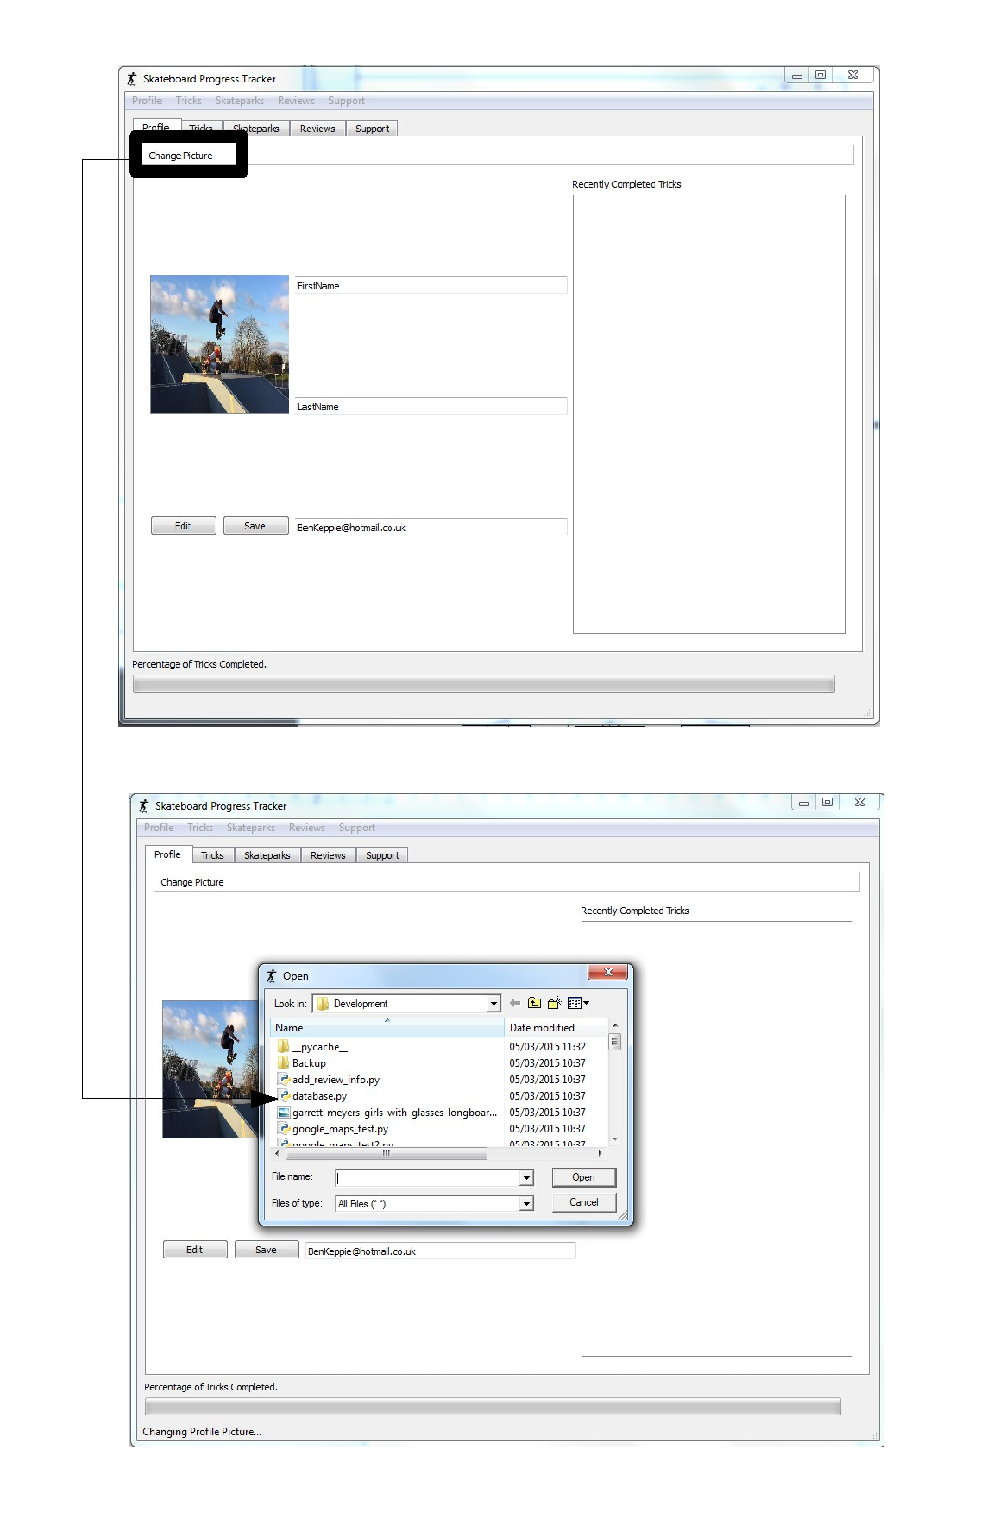
\includegraphics[width=\textwidth]{./Maintenance/Figures/ChangePicture.pdf}
    \caption{User interface, changing profile picture} \label{fig:Changing Picture UI}
\end{figure}


\begin{figure}[H]
    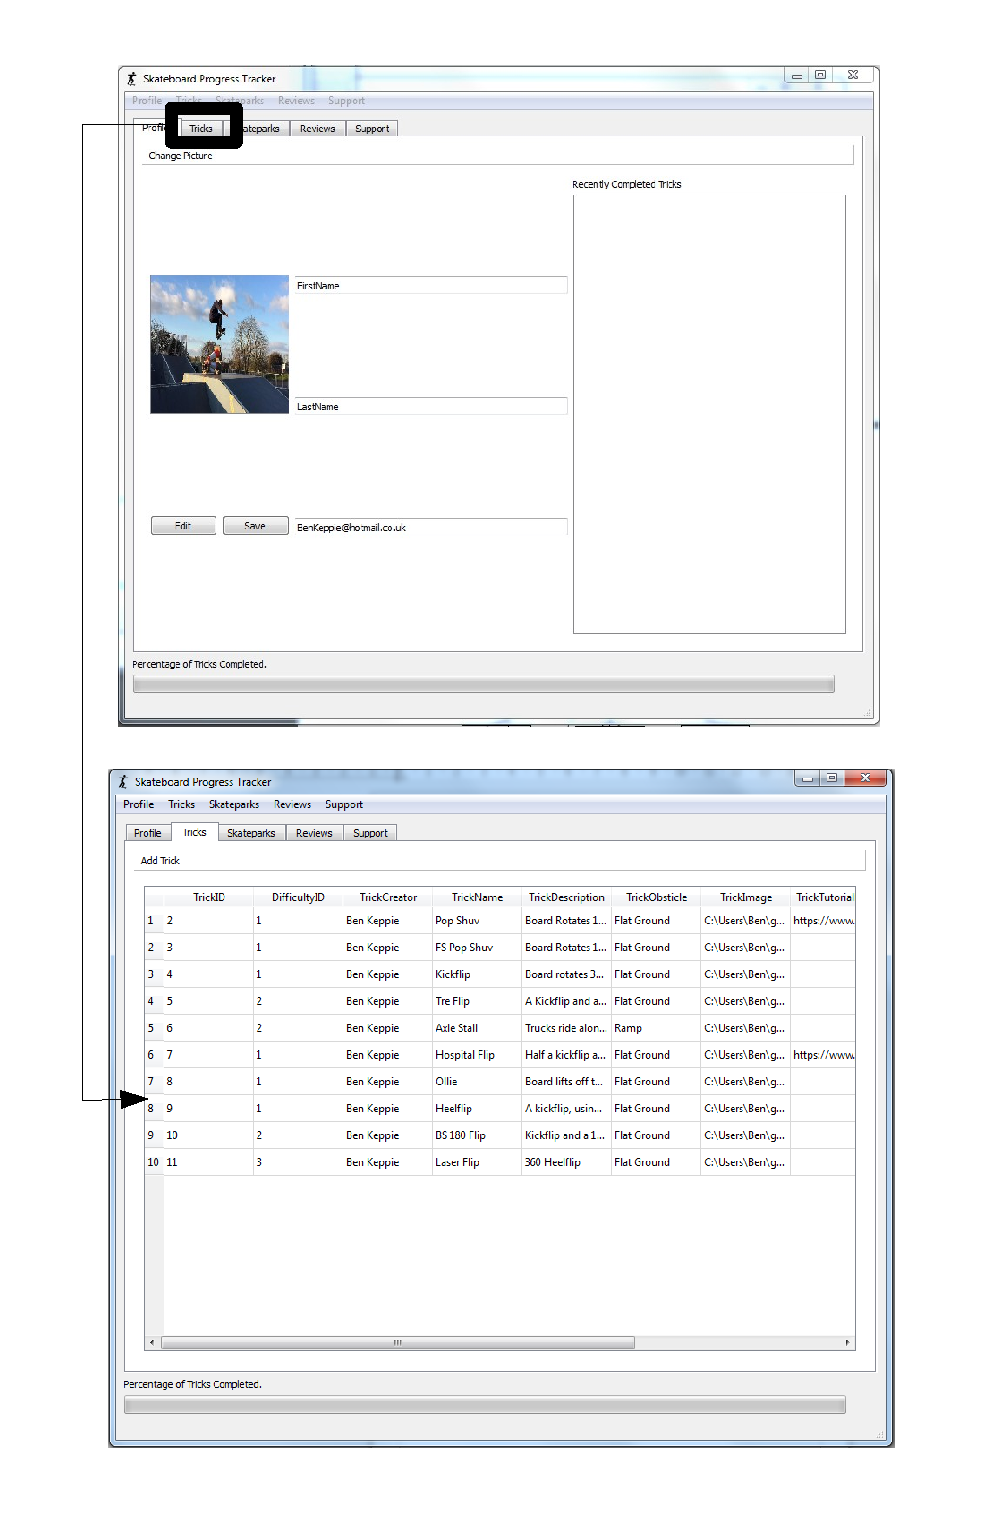
\includegraphics[width=\textwidth]{./Maintenance/Figures/TricksTab.pdf}
    \caption{User interface, switching to the tricks tab} \label{fig:Trick Tab UI}
\end{figure}


\begin{figure}[H]
    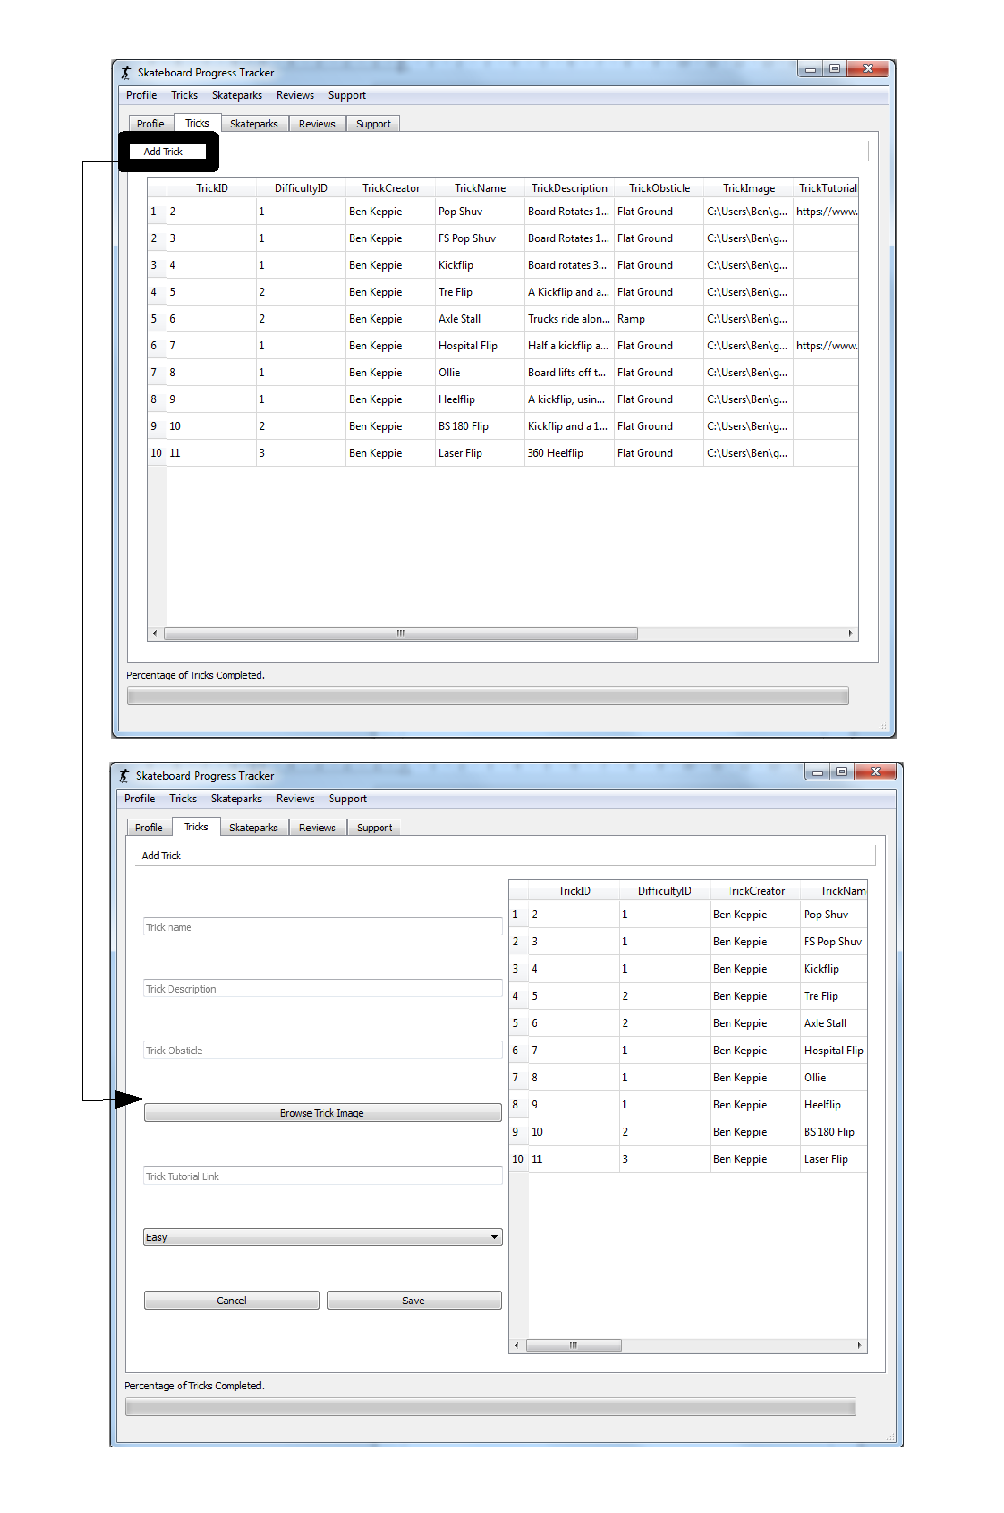
\includegraphics[width=\textwidth]{./Maintenance/Figures/AddTrick.pdf}
    \caption{User interface, adding a trick} \label{fig:Add Trick UI}
\end{figure}


\begin{figure}[H]
    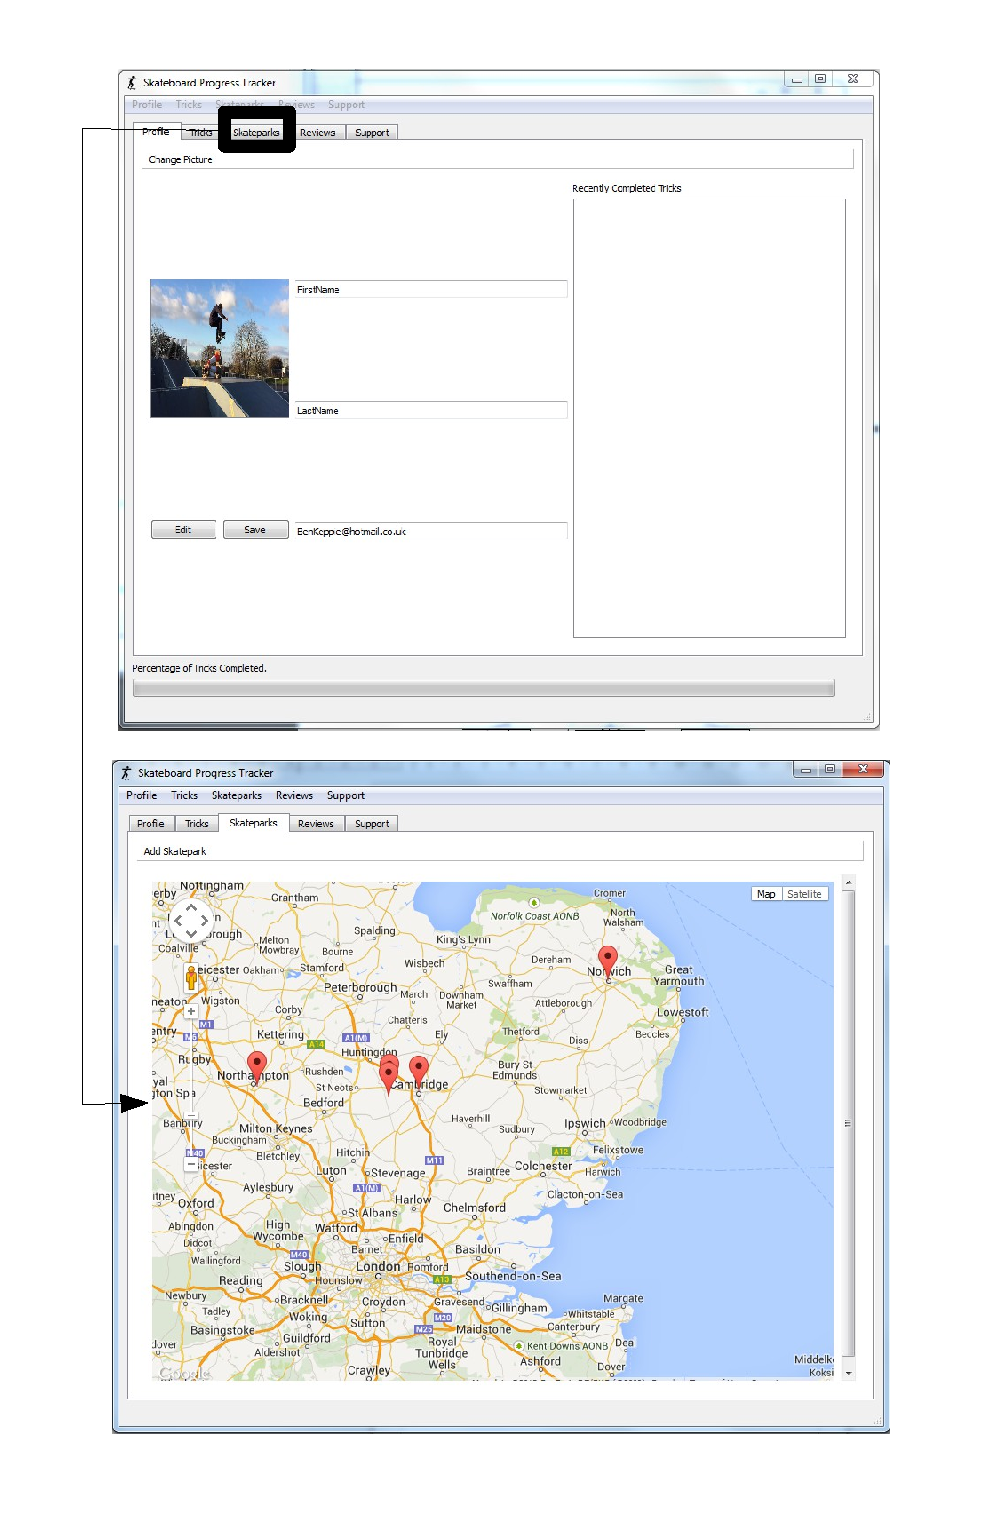
\includegraphics[width=\textwidth]{./Maintenance/Figures/SkateparkTab.pdf}
    \caption{User interface, switching to the skateparks tab} \label{fig:Skatepark Tab UI}
\end{figure}


\begin{figure}[H]
    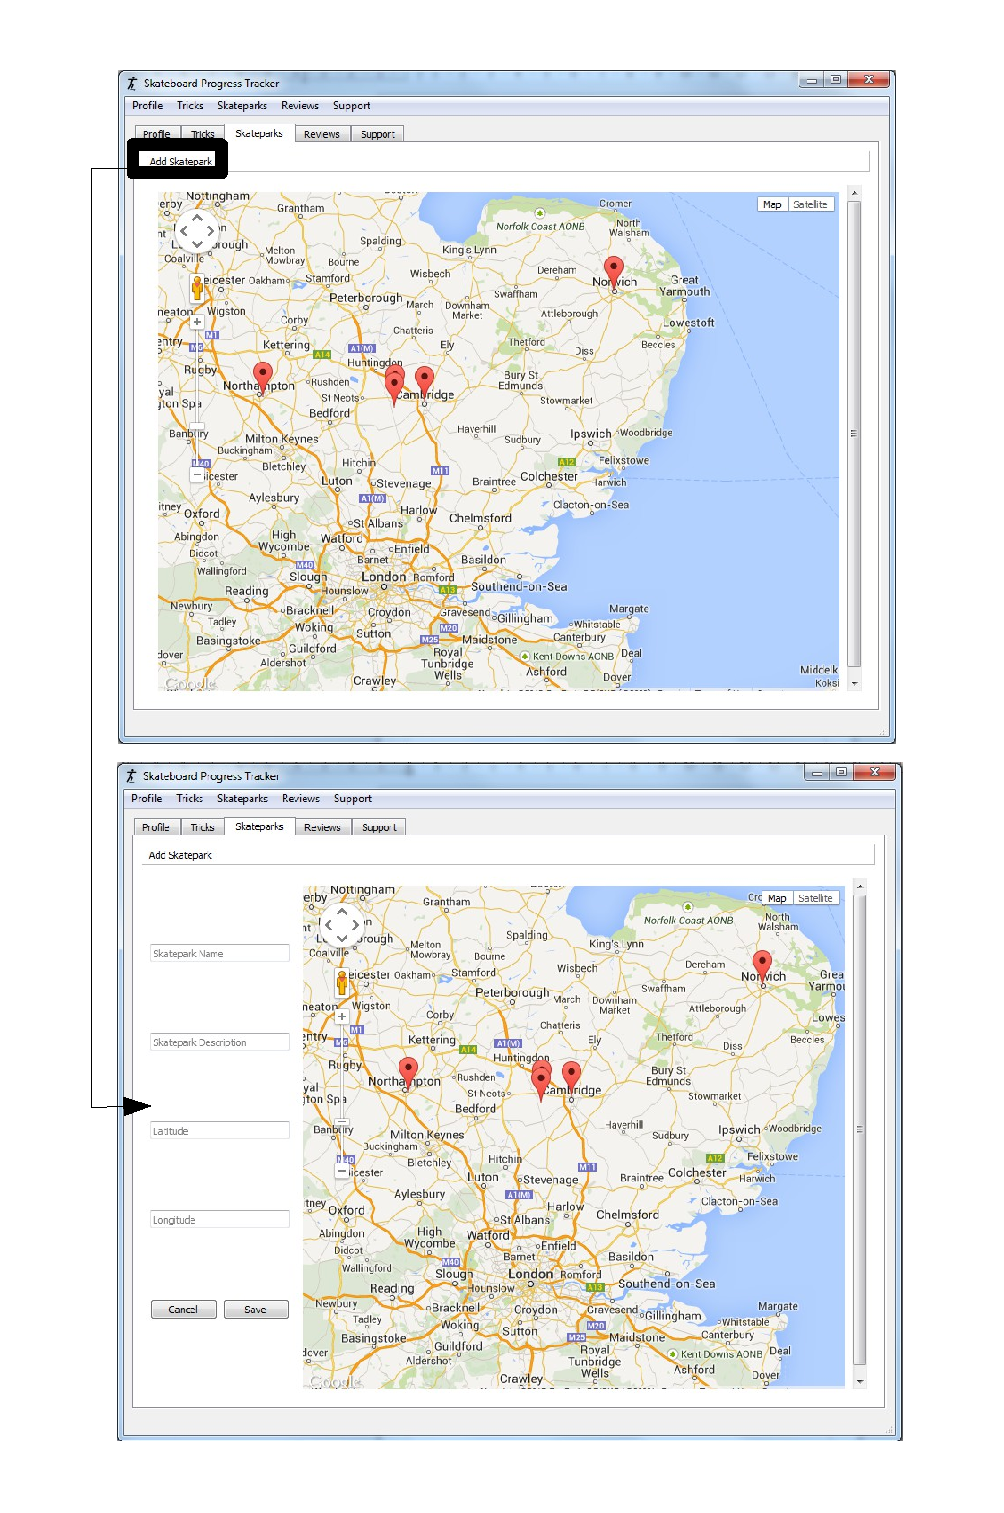
\includegraphics[width=\textwidth]{./Maintenance/Figures/AddSkatepark.pdf}
    \caption{User interface, adding a skatepark} \label{fig:Add Skatepark UI}
\end{figure}


\begin{figure}[H]
    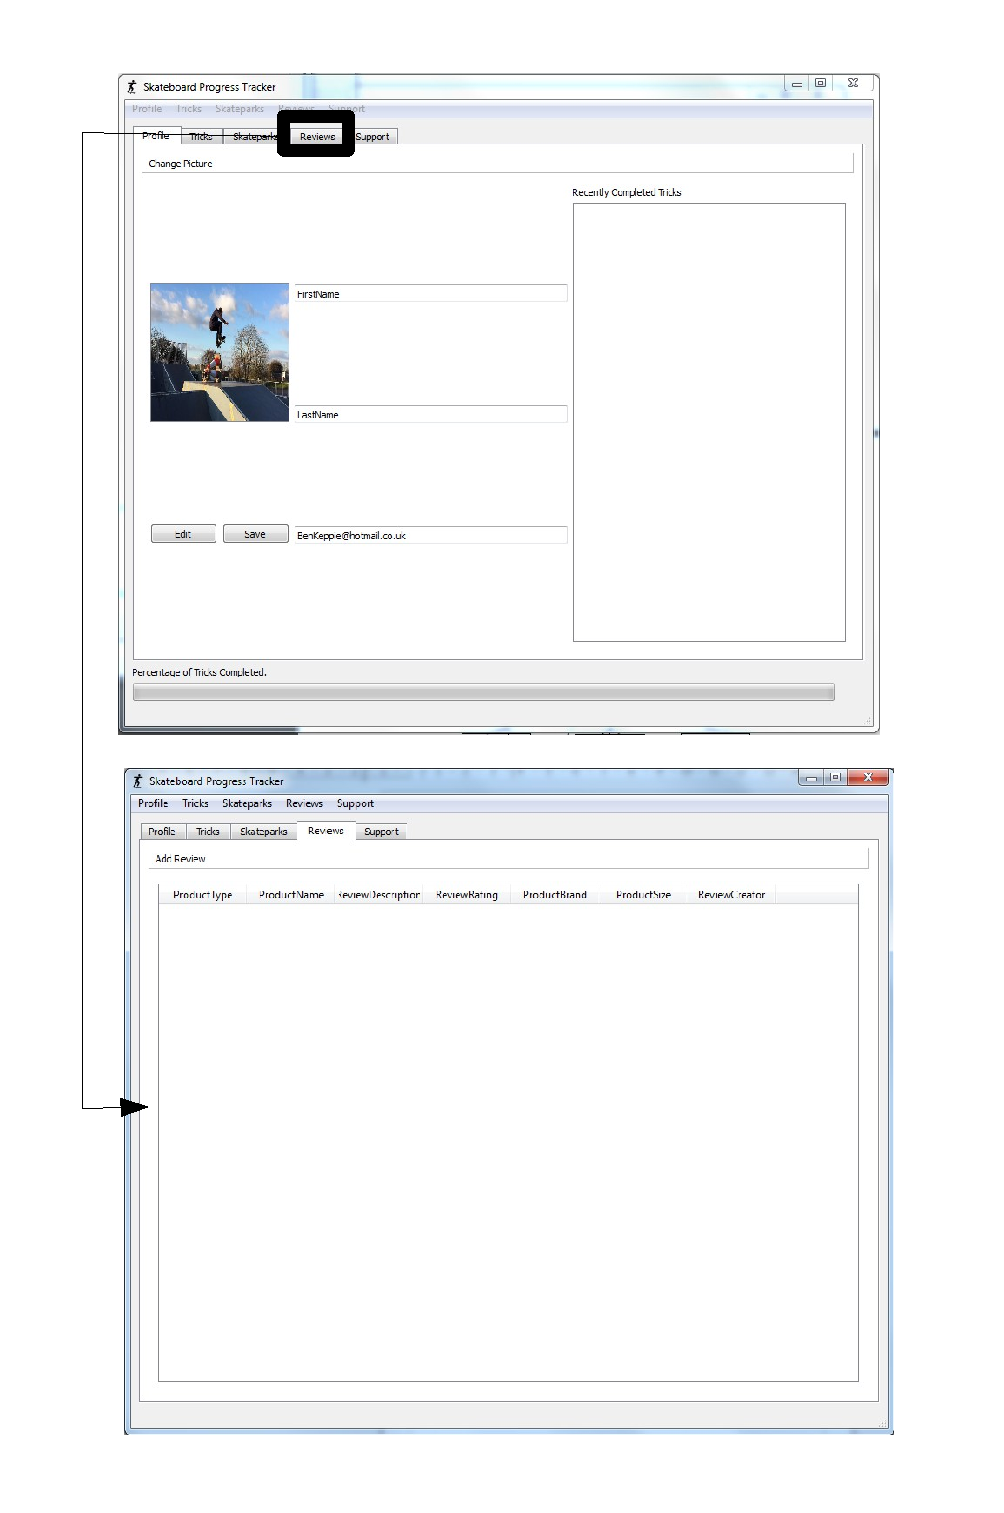
\includegraphics[width=\textwidth]{./Maintenance/Figures/ReviewTab.pdf}
    \caption{User interface, switching to the reviews tab} \label{fig:Review Tab UI}
\end{figure}


\begin{figure}[H]
    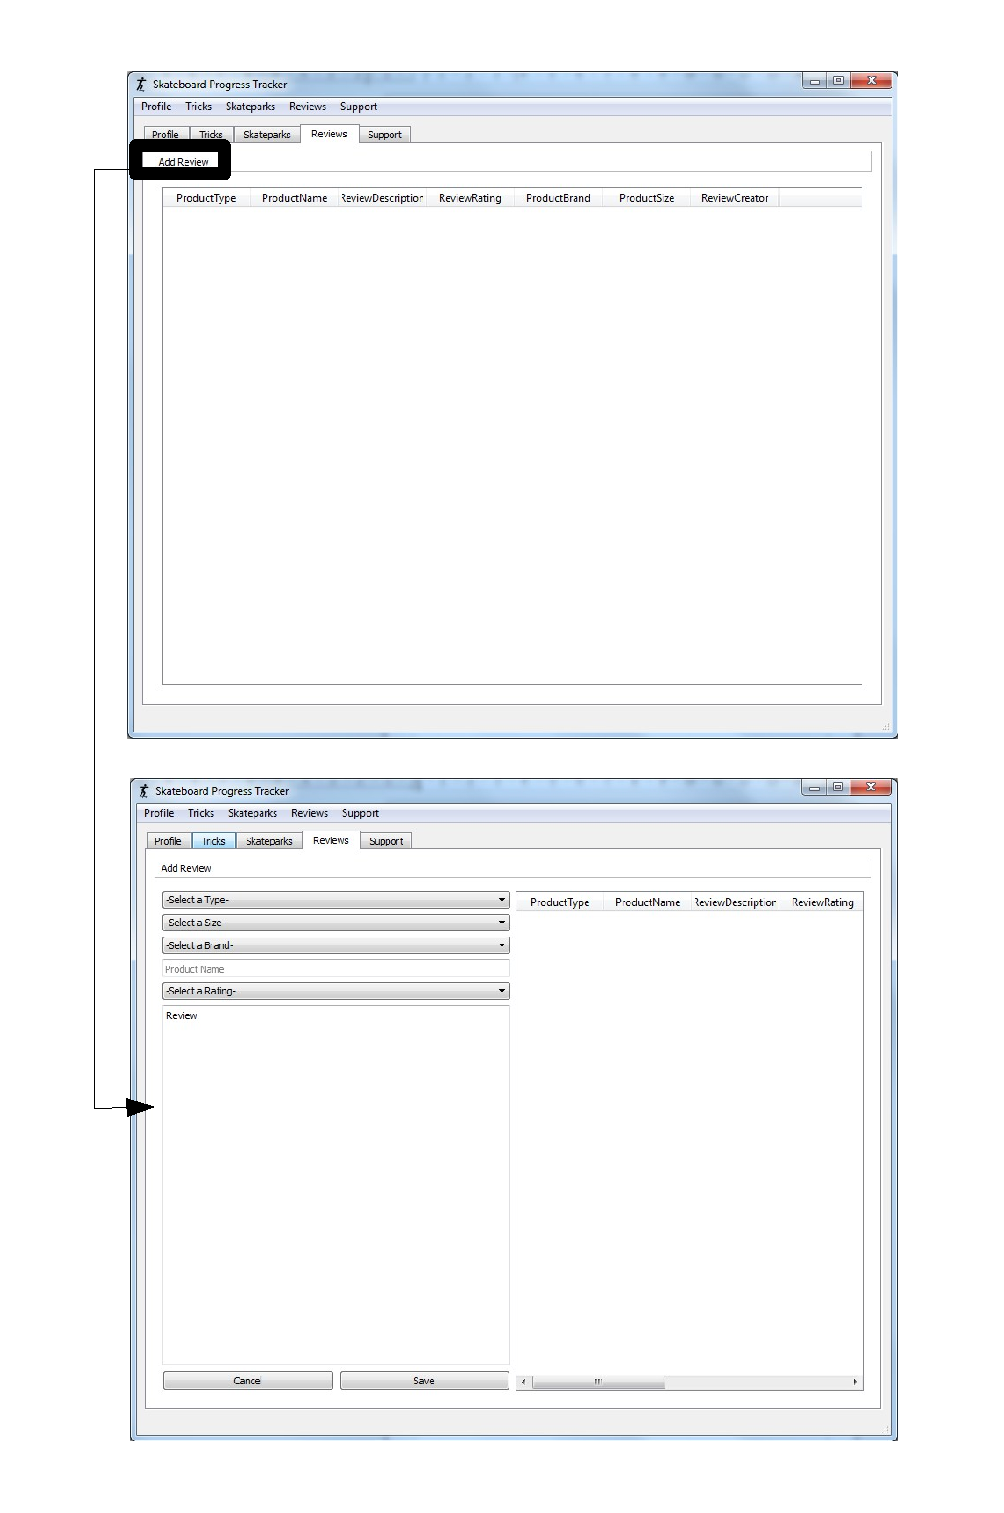
\includegraphics[width=\textwidth]{./Maintenance/Figures/AddReview.pdf}
    \caption{User interface, adding a review} \label{fig:Add Review UI}
\end{figure}


\begin{figure}[H]
    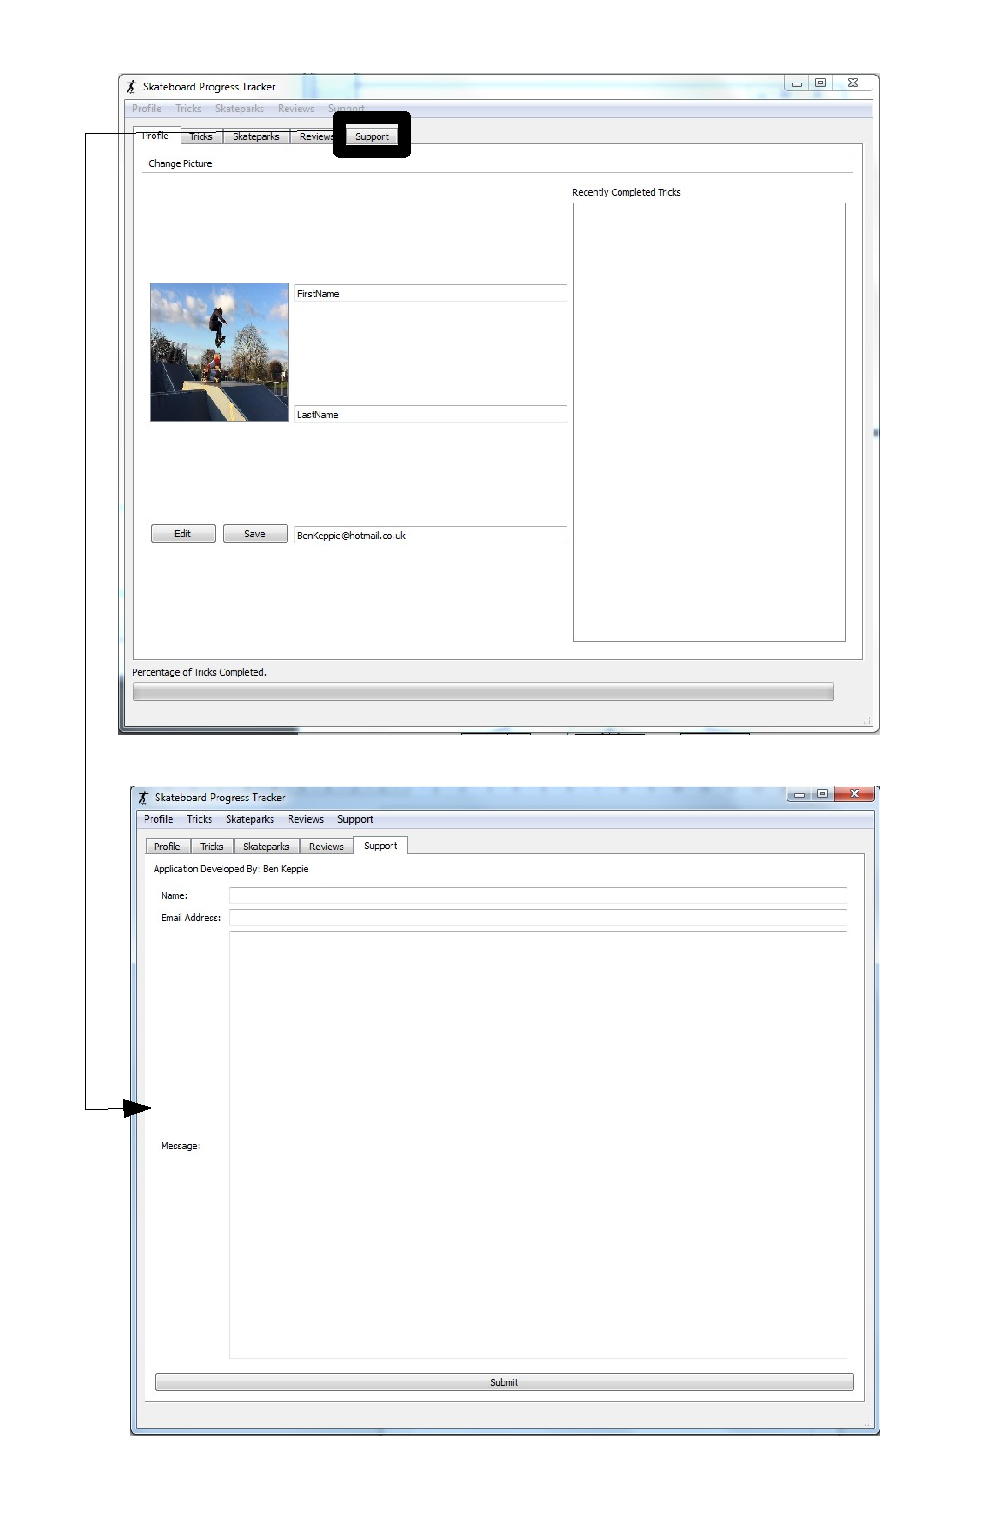
\includegraphics[width=\textwidth]{./Maintenance/Figures/SupportTab.pdf}
    \caption{User interface, switching to the support tab} \label{fig:Support Tab UI}
\end{figure}











\subsection{ER Diagram}

\begin{figure}[H]
    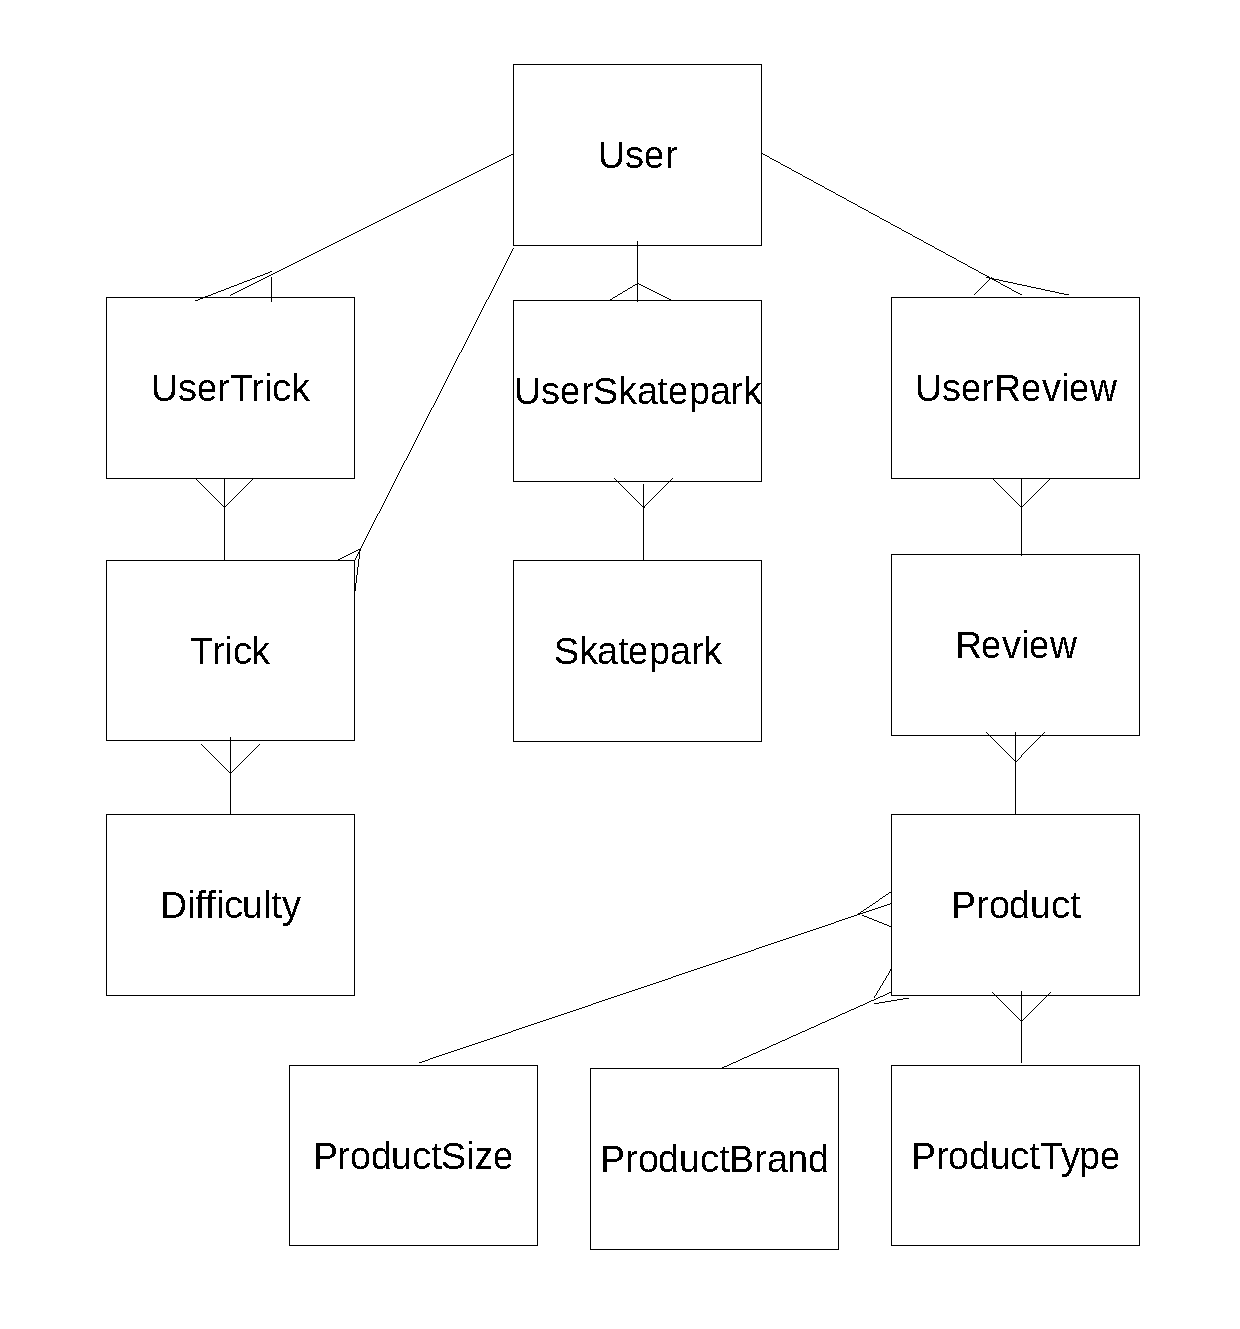
\includegraphics[width=\textwidth]{./Design/EntityRelationships2.pdf}
    \caption{Entity-Relationship Diagram} \label{fig:Entity Diagram}
\end{figure}







\subsection{Database Table Views}

\begin{figure}[H]
    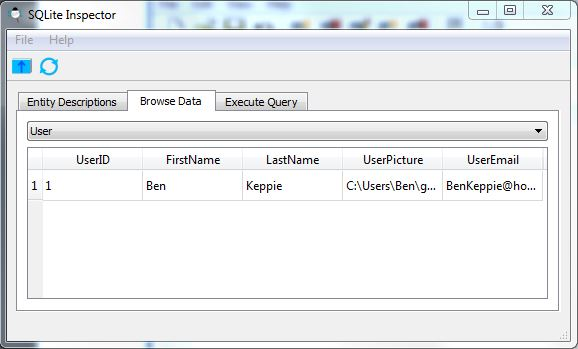
\includegraphics[width=\textwidth]{./Maintenance/Figures/UserTable.jpg}
    \caption{The user table of the database} \label{fig:User Table}
\end{figure}

\begin{figure}[H]
    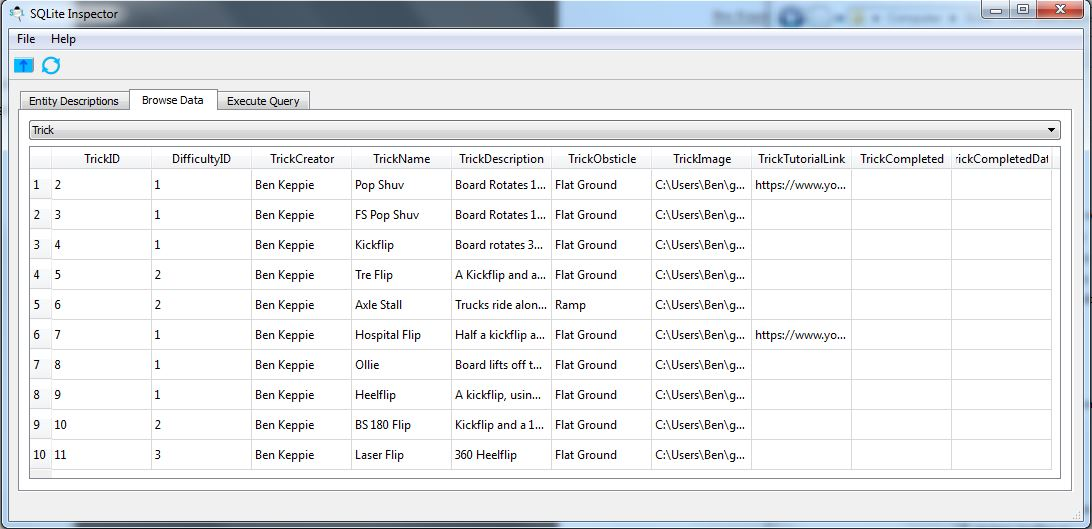
\includegraphics[width=\textwidth]{./Maintenance/Figures/TrickTable.jpg}
    \caption{The trick table of the database} \label{fig:Trick Table}
\end{figure}


\begin{figure}[H]
    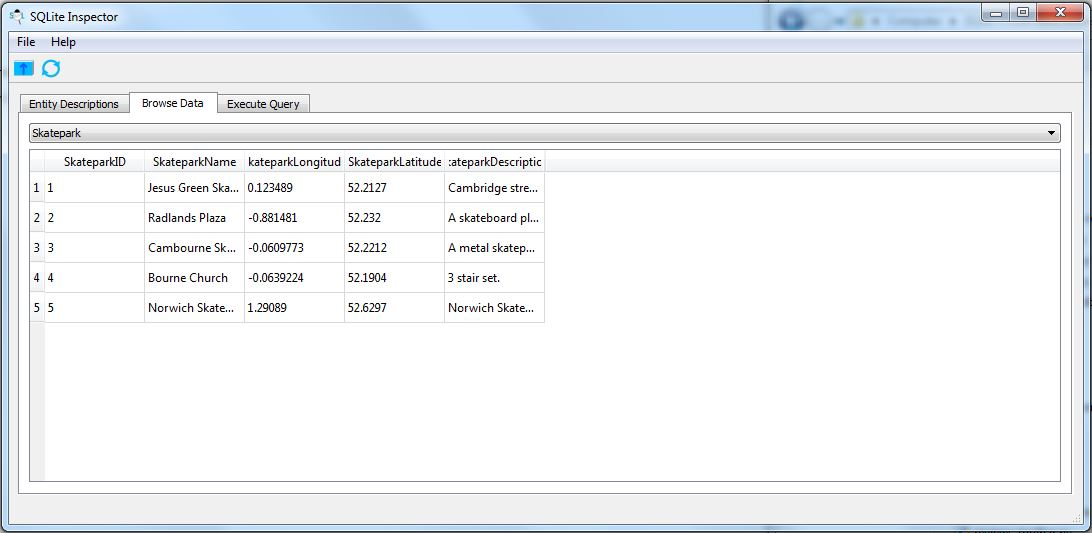
\includegraphics[width=\textwidth]{./Maintenance/Figures/SkateparkTable.jpg}
    \caption{The skatepark table of the database} \label{fig:Skatepark Table}
\end{figure}

\begin{figure}[H]
    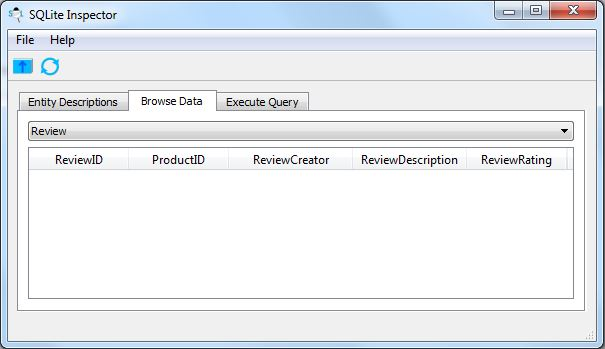
\includegraphics[width=\textwidth]{./Maintenance/Figures/ReviewTable.jpg}
    \caption{The review table of the database} \label{fig:Review Table}
\end{figure}

\begin{figure}[H]
    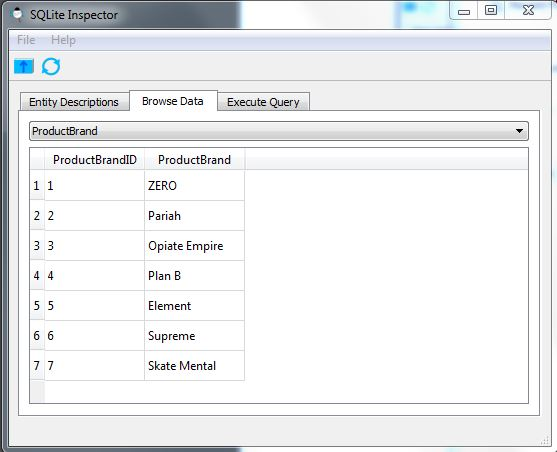
\includegraphics[width=\textwidth]{./Maintenance/Figures/ProductBrandTable.jpg}
    \caption{The product brand table of the database} \label{fig:ProductBrand Table}
\end{figure}

\begin{figure}[H]
    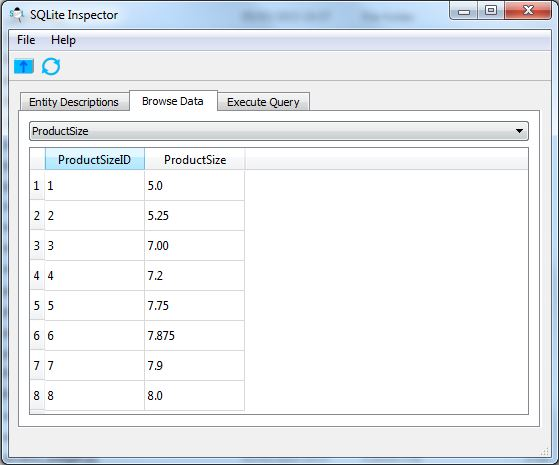
\includegraphics[width=\textwidth]{./Maintenance/Figures/ProductSizeTable.jpg}
    \caption{The product size table of the database} \label{fig:ProductSize Table}
\end{figure}

\begin{figure}[H]
    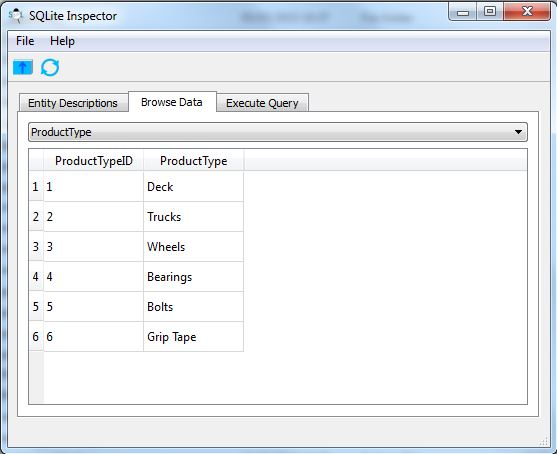
\includegraphics[width=\textwidth]{./Maintenance/Figures/ProductTypeTable.jpg}
    \caption{The product type table of the database} \label{fig:ProductType Table}
\end{figure}

\subsection{Database SQL}

To create the entities I used the following SQL code:

\pythonfile[firstline=28, lastline=105]{./Implementation/CLI/database.py}

\subsection{SQL Queries}

\section{Testing}

\subsection{Summary of Results}

\subsection{Known Issues}

\section{Code Explanations}

\subsection{Difficult Sections}

\subsection{Self-created Algorithms}

\section{Settings}






\section{Acknowledgements}

\begin{itemize}
\item Acknowledgment 1 - YouTube link regular expression - Found on \url{http://stackoverflow.com/questions/3717115/regular-expression-for-youtube-links} by Stack Overflow user \url{http://stackoverflow.com/users/3652125/fanmade}
\item Acknowledgment 2 - Google Maps JavaScript API - Gained from Google's APIs Console. - \url{https://developers.google.com/maps/documentation/javascript/tutorial}
\item Acknowledgment 3 - Javascript help on Stack Overflow - \url{http://stackoverflow.com/questions/28253168/running-a-javascript-function-from-qwebview-google-maps-api-pyqt} I posted a question to attempt to resolve an issue I had with my Javascript code.
\end{itemize}

\section{Code Listing}

\subsection{Main Window}

\pythonfile[firstline=1]{./Implementation/main_window.pyw}

\subsection{Main Tabbed Widget}

\pythonfile[firstline=1]{./Implementation/main_tab_widget.py}

\subsection{Menu Bar}

\pythonfile[firstline=1]{./Implementation/menu_bar.py}



\subsection{Profile Widget}

\pythonfile[firstline=1]{./Implementation/profile_widget.py}

\subsection{Profile Picture}

\pythonfile[firstline=1]{./Implementation/profile_picture.py}

\subsection{Profile Toolbar}

\pythonfile[firstline=1]{./Implementation/profile_toolbar.py}

\subsection{Profile SQL Connections}

\pythonfile[firstline=1]{./Implementation/profile_sql_connections.py}



\subsection{Tricks Widget}

\pythonfile[firstline=1]{./Implementation/tricks_widget.py}

\subsection{Tricks Toolbar}

\pythonfile[firstline=1]{./Implementation/tricks_toolbar.py}

\subsection{Tricks SQL Connections}

\pythonfile[firstline=1]{./Implementation/tricks_sql_connections.py}



\subsection{Skateparks Widget}

\pythonfile[firstline=1]{./Implementation/skateparks_widget.py}

\subsection{Skateparks Map}

\pythonfile[firstline=1]{./Implementation/skatepark_view_only.py}

\subsection{Skateparks Toolbar}

\pythonfile[firstline=1]{./Implementation/skateparks_toolbar.py}

\subsection{Skateparks SQL Connections}

\pythonfile[firstline=1]{./Implementation/skateparks_sql_connections.py}



\subsection{Reviews Widget}

\pythonfile[firstline=1]{./Implementation/reviews_widget.py}

\subsection{Reviews Toolbar}

\pythonfile[firstline=1]{./Implementation/reviews_toolbar.py}

\subsection{Reviews SQL Connections}

\pythonfile[firstline=1]{./Implementation/reviews_sql_connections.py}



\subsection{Support Widget}

\pythonfile[firstline=1]{./Implementation/support_widget.py}



\subsection{CLI Menu}

\pythonfile[firstline=1]{./Implementation/CLI/menu.py}

\subsection{CLI Get Menu Option}

\pythonfile[firstline=1]{./Implementation/CLI/get_menu_option.py}

\subsection{CLI Database Table Menu}

\pythonfile[firstline=1]{./Implementation/CLI/database_table_menu.py}

\subsection{CLI Create Database}

\pythonfile[firstline=1]{./Implementation/CLI/database.py}

\subsection{CLI Profile Edit Options}

\pythonfile[firstline=1]{./Implementation/CLI/profile_edit_options.py}

\subsection{CLI Trick Edit Options}

\pythonfile[firstline=1]{./Implementation/CLI/trick_edit_options.py}

\subsection{CLI Skatepark Edit Options}

\pythonfile[firstline=1]{./Implementation/CLI/skatepark_edit_options.py}

\subsection{CLI Review Edit Options}

\pythonfile[firstline=1]{./Implementation/CLI/review_edit_options.py}

\subsection{CLI Make New Difficulty}

\pythonfile[firstline=1]{./Implementation/CLI/difficulty.py}

\subsection{CLI Make New Product}

\pythonfile[firstline=1]{./Implementation/CLI/products.py}




